\documentclass[10pt,twocolumn,letterpaper]{article}

%% Language and font encodings
\usepackage[spanish,english]{babel}
\usepackage[utf8x]{inputenc}
\usepackage[T1]{fontenc}

%% Sets page size and margins
\usepackage[a4paper,top=3cm,bottom=2cm,left=3cm,right=3cm,marginparwidth=1.75cm]{geometry}

%% Useful packages
\usepackage{amsmath}
\usepackage{graphicx}
\usepackage[colorinlistoftodos]{todonotes}
\usepackage[colorlinks=true, allcolors=blue]{hyperref}
\setlength{\marginparwidth}{2cm}

%% Title
\title{
		%\vspace{-1in} 	
		\usefont{OT1}{bch}{b}{n}
		\normalfont \normalsize \textsc{CSC-370A Data Mining} \\ [14pt]
		\huge Housing Price Prediction Model \\
}

\usepackage{authblk}
\author[1]{Ahmed Kaleem Chaudhry (achaudhry-2022@depauw.edu) Muhammad Moeez Khan (mkhan-2024@depauw.edu)}


\begin{document}
\maketitle

\selectlanguage{english}

\begin{abstract}
The objectives of this work revolves around fine-tuning the data set for the model developed and using machine learning techniques to produce accurate forecasts for housing prices. This guide gives step-by-step instructions on how to adjust the data set such that prediction models fit it perfectly before utilizing various models to anticipate initially unobserved housing data. In order to pre-process the data, missing information had to be filled in, features had to be created, and outliers had to be found.\end{abstract}


\section{Keywords:}
Some keywords for this project include  Gradient Boosting Regressor, KNN Regressor, Linear Regression, Feature Engineering, KNN Imputer, and Scaling.

\section{Introduction:}
This paper presents a comprehensive study on the use of machine learning techniques for predicting the prices of residential properties in a specific location. The authors carefully preprocessed the dataset by cleaning and preparing the data, and then used a variety of predictive models to build their prediction model. After extensive experimentation, the authors found that the best results were obtained using an ensemble technique called stacking, which combined the predictions of multiple models to improve the accuracy and robustness of the final model. The paper discusses the various steps taken and the results obtained in detail, providing insights and lessons learned that can be useful for others working on similar problems.

\section{Preprocessing:}
"Preprocessing" the data is the most crucial step before testing our data and is very important in the data analysis process in pandas. Preprocessing refers to the process of cleaning, transforming, and preparing data for further analysis. One of the key reasons why we focused majorly on preprocessing pertained to how it allowed us to make sure that our data is in a format that is suitable for the type of preferred analysis. For example, when we wanted to run a regression analysis, we needed to make sure that our data is in a format that is compatible with regression algorithms. Preprocessing helped us convert our data into the correct format, and also helped us identify and remove any missing or invalid data points.

\subsection{Feature Engineering:}
Feature engineering is an important step in the data analysis and machine learning process since it involves transforming raw data into features that can be used to build predictive models. Some aspects of Feature Engineering that we utilized were extracting useful features from raw data, combining existing components to create new ones, and selecting a subset of the most relevant features to use in a model.

In pandas, feature engineering can be performed using a variety of methods and techniques. For example, we may one-hot encode attributes by using the "get-dummies" method of the pandas module. With one-hot encoding, each distinct integer value essentially introduces a new binary variable. Our dataset may become more dimensional, but it is better suited for machine learning because the labels are unrelated to one another. The following are the 4 methods we utilized to convert categorical data into numeric data.
\begin{itemize}
    \item convertOrdinal → manually converts ordinal data into numeric data using map()
    \item dropNominal → drops all the nominal data types
    \item convertNominalBinary → converts the binary nominal values into 0s and 1s
    \item convertNominalMulticlass → converts all the rest of the nominal values into numeric data
\end{itemize}

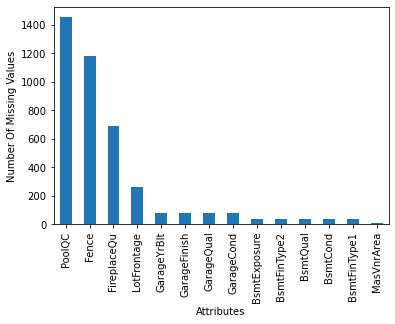
\includegraphics[width=6.5cm,height=7cm]{plot#4 - missing value stats.png}
Figure 1 - The Attributes With The Most Missing Values In A Line Graph
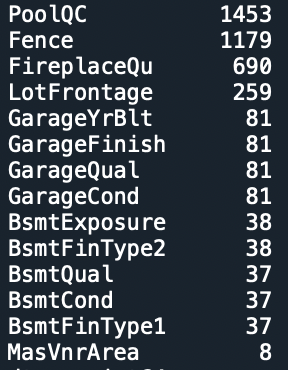
\includegraphics[width=7cm,height=6cm]{Screen Shot 2022-12-15 at 6.15.02 AM.png}
Figure 2 - The Attributes With The Most Missing Values With Exact Values
\subsection{Missing Values:}
Dealing with missing values is important when working with data in pandas for several reasons. First, many machine learning algorithms cannot handle missing values and will either produce an error or produce incorrect results if they encounter missing values in the data. Second, even if a particular algorithm can handle missing values, the presence of missing values in our data can still affect the accuracy of the results. And third, missing values initially made it difficult to understand and interpret our data, which could have possibly hindered our ability to make informed decisions based on the data. 

As shown in Figure.1 for our project's attributes, PoolQC (pool quality) has 1453 missing data, Fence has over 1179, and there are many more characteristics with a large proportion of missing values. This illustrates how crucial it is to deal with missing values since they may prevent some processes from working or result in unexpected outcomes. For instance, if a DataFrame has missing values, only the non-missing values will be used to determine the mean of the columns, which may not adequately reflect the data.

Moreover, as we progressed with the project's development and faced bugs, our debugging process got easier since no missing values were causing confusion and making it difficult for us to understand the data. For example, if we tried to analyze the dataset and some of the values were missing, it was difficult to determine whether the missing values contributed to the error at hand.

The KNN imputer is a missing value imputation method that uses the K-Nearest Neighbors algorithm to fill in missing values in a dataset. There are a couple of ways to deal with missing values. We used the scikit-learn module Imputer, where we used it to fill in the missing values for additional variables that had some missing values. By default, the Imputer attempts to fill in the gaps in the data by using a mean value. This approach can also be changed to the median or mode, which will be investigated in subsequent studies. However, we were unable to delve into this due to time constraints.

The module finds the k-nearest neighbors of each row by measuring the separation between the rows in the dataset. The mean or median of the attribute values of the k-nearest neighbors is then used to impute the missing values in each row.

\begin{itemize}
    \item findMissingValueStats → Find the Number of Missing Values For Each Attribute
    \item fillMissingValuesWithMean → Fill in the Missing Values With the Field's Mean Value
    \item fillMissingValuesWithMode → Fill in the Missing Values With the Field's Mode Value
    \item fillMissingValuesWithMedian → Fill in the Missing Values With the Field's Median Value
    \item fillMissingValuesWithKNNImputer → Fill in the Missing Values With The 'K' Nearest Neighbors' Mean Value 
    \item dropMissingValues → Drop All Attributes That Have Missing Values
\end{itemize}


\subsection{Scaling Data:}
Scaling is an important preprocessing step in data analysis and machine learning. In general, the goal of scaling is to transform the data so that it has a similar scale across all features. This is important because many machine learning algorithms, including most distance-based algorithms, are sensitive to the relative scales of the features in the data.

When using distance-based computations, such as those used in our K-Nearest Neighbor implementation, one feature in a dataset took precedence over other features if it has a considerably wider range of values than the others. The algorithm may thus produce less-than-ideal or even inaccurate results as a result. Scaling the data made it easier for us to make sure that all attributes are given the same weight in the computations, which can enhance the algorithm's efficiency and precision.

\begin{itemize}
    \item normalize → We performed normalization on a Dataframe using the standard 'loc' and higher-order 'max' and 'min' functions and the formula.
    \item standardize → We performed standardization on a DataFrame using the standard 'loc' and higher-order 'mean' and 'std'(standard deviation) functions and the formula.
\end{itemize}


\subsection{Outlier Values:}
Removing outlying values, also known as "outlier detection" or "outlier removal," is an important preprocessing step in data analysis and machine learning. Outliers are data points that lie outside the expected range of values for a given variable. The importance of outlier removal lies in its ability to improve the performance and accuracy of machine learning models. Outliers can have a disproportionately large effect on the results of an analysis, and can sometimes cause algorithms to produce incorrect or misleading results. By removing outliers, we ensured that the data used to build a model is more representative of the underlying distribution of the data, which can lead to better and more reliable results.

To find outlier values in a pandas DataFrame using z-scores, we used the z-score method from the scipy.stats library. This method calculates the z-score for each value in the data, which is a measure of how many standard deviations a given value is from the mean. Outliers typically have a z-score that is greater than 3 or less than -3 (something we learned in our statistics classes), so we used these thresholds to identify outlying values in the data.
\begin{itemize}
    \item dropOutlierRows → Drop All Rows That Have Outlier Values For Any Attributes
\end{itemize}


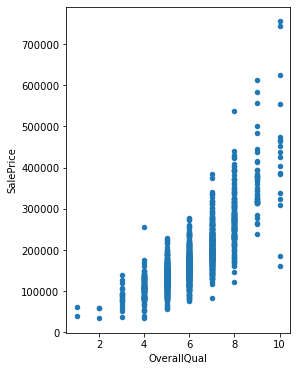
\includegraphics[width=8cm,height=8cm]{plot#5 - highest corelation.png}
Figure 3 - The Correlation between "OverallQuall" and "SalePrice", we chose to find the correlation between "OverallQuall" since it proved to be the most correlated attribute (as illustrated in Figure.5)
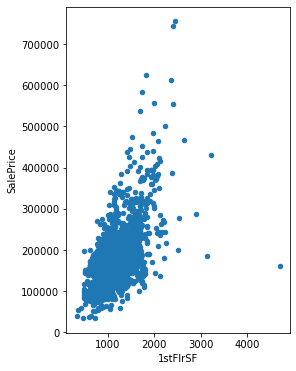
\includegraphics[width=8cm,height=8cm]{plot#3 - attribute2 corelation.png}
Figure 4 - The Correlation between "1stFlrSF" and "SalePrice", we chose to find the correlation between "1stFlrSF" since it was used as a predictor in the given code.
\subsection{Co-Relation:}
We found using correlated techniques in pandas to be helpful since they allowed us to find patterns and correlations in the given data. For instance, a strong correlation between two variables might mean that they are likely to change in tandem in controlled situations. This was useful for identifying the underlying links between various parameters in our dataset and for forecasting the future values of our data. Additionally, avoiding overfitting our model, which can improve performance on fresh, untested data, was made possible by the use of correlated approaches.

Furthermore, because they assisted us in seeing patterns and correlations in our data, using correlated values as predictors in pandas might be advantageous. For instance, having two variables with a high degree of correlation \textbf{}y mean that they are likely to change in tandem in predictable ways. This assisted us in understanding the underlying links between the many variables in our dataset and in making predictions about future values. Additionally, by avoiding overfitting our model, which might improve performance on fresh, untested data, we were able to avoid utilizing correlated values as predictors.

\begin{itemize}
    \item kHighestCorelatedAttributes → Find the Attributes that Are Highly Co-Related With the "SalePrice" and Treat Them As Predictors
\end{itemize}



\section{Algorithms:}
\textbf{Linear regression}, \textbf{KNN Regressor}, and \textbf{Gradient Boosting Regressor (GBR)} are three different types of machine learning algorithms that we used for predicting housing prices.

Linear regression is a simple and widely used technique for predicting a continuous variable, such as housing prices. It assumes that there is a linear relationship between the input variables and the output variable, and uses this relationship to make predictions.

KNN Regressor, on the other hand, is a non-parametric method that makes predictions based on the similarity of the input data to other data points in the training set. It is a lazy learning algorithm, which means that it does not learn a model from the training data, but instead makes predictions based on the training data directly.

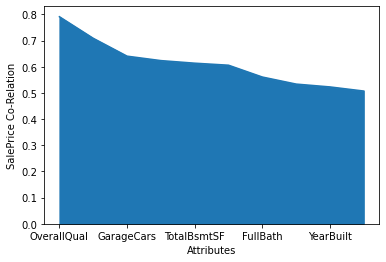
\includegraphics[width=7cm,height=7cm]{img1.png}
Figure 5 - The Attributes With The Highest Correlations With "SalePrice"

Gradient Boosting Regressor is an ensemble learning method that combines multiple weak learners to create a strong predictor. It works by sequentially training weak learners to correct the mistakes of the previous learners, and then combining them to produce a final prediction.


Overall, linear regression is a simple and fast method for making predictions, but it can only model linear relationships and may not be accurate for complex data. Especially, in our case, the model's performance was not that good and only peaked at '0.7453'. Similarly, KNN Regressor through a flexible and effective algorithm, but was too slow to make predictions and did not work well since we have high-dimensional data. However, the accuracy of this model slowly increased when we fit it to the prepossessed data, which utilized techniques like standardization and normalization, rather than raw data. Eventually, it peaked at around '0.72747' from '0.640'. 

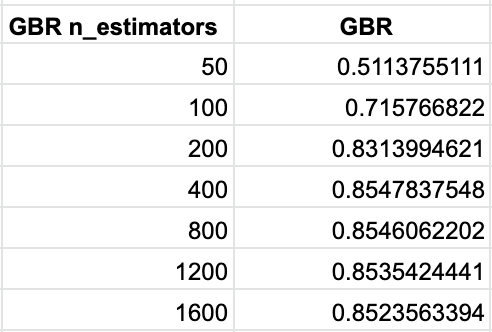
\includegraphics[width=6.5cm,height=6cm]{Screen Shot 2022-12-15 at 6.41.42 AM.png}
Figure 6 - The Changes In Accuracy Of The GBR Algorithm With Parameter Tuning Of "n-estimators" Attribute


Meanwhile, the Gradient Boosting Regressor was the clear winner because of its  powerful and accurate method. It had a pretty good accuracy from the very start but upon testing and hypothesizing we realized that there was still room for improvement. We tuned its parameter. And of course, the accuracy increased. It increased from '0.715' with 'n-estimators' = 100 to '0.854' with 'n-estimators' = 400. We found the optimal value of its parameter for which it gave the best result. However, there are also some drawbacks to this model. The model  can be difficult to tune and may require a lot of computational resources.


\section{Results:}
Our top Kaggle score was 0.26157, which placed us 3915th out of 4619 users.




\section{Future Work:}
More sophisticated algorithms such as Deep Neural Networks and Advanced Gradient Boosting could be explored. Additionally, other feature engineering techniques and pre-processing might be able to improve our score. 


\section{Conclusion:}
The method of projecting home prices from the Housing Dataset is examined in this study, along with the many strategies we utilized. The given dataset had a number of problems, namely: missing values, inaccurate data, and some irrelevant data. Thus, in order to clean the data, we used a variety of techniques and procedures. Examples of crucial components of our pre-processing that enhanced our forecasts include feature engineering, eliminating missing data, deleting outliers, etc. We also tested a wide range of methods, such as Gradient Boosting Regressor, Linear Regression, Knn regressor. After doing a variety of tests, we discovered that the GBR generated the best results. 

\bibliographystyle{vancouver}
\bibliography{references}
contactsunny.medium.com/label-encoder-vs-one-hot-encoder-in-machine-learning-3fc273365621\\

youtube.com/watch?v=CtVr5aMHL7Y\\

blog.paperspace.com/implementing-gradient-boosting-regression-python/\\

datatechnotes.com/2019/06/gradient-boosting-regression-example-in.html\\

datatechnotes.com/2019/04/regression-example-with-k-nearest.html\\

stackoverflow.com/questions/23199796/detect-and-exclude-outliers-in-a-pandas-dataframe\\

betterdatascience.com/impute-missing-data-with-python-and-knn/
\end{document}